\section{Deanonymization Attacks and Their Implications} \label{sec:attacks}
In this section we survey deanonymization attacks on Bitcoin users. Such attacks can be roughly characterized into the following four categories based on the source of information used to carry out the attack:
\begin{enumerate}
	\item Multi-input transaction attacks,
	\item Bitcoin value flow attacks,
	\item Implementation-specific side channel attacks that rely on timing and network-layer (e.g., IP addresses) information, and
	\item Auxiliary information linkability attacks (e.g., entity-to-address linking using information acquired via external mediums).
\end{enumerate}
Our analysis is based on the small body of work primarily analyzing the first three classes of attacks. The last class is generally not discussed in scholarly work, but rather in popular media. Before discussing any attacks, we first describe the attack vectors leveraged by malicious users and researchers while conducting such attacks.

\subsection{Attack Vectors} \label{sec:vectors}
Given the design of the Bitcoin system, it may seem surprising that the surface for deanonymization attacks is quite large. In fact, there is a large amount of information available to attackers that may be, and has been, exploited to carry out such attacks. We discuss only a few here. Perhaps most fruitful are the \emph{transaction} and \emph{user} graphs that can be constructed via network and transaction analysis. The transaction graph is a directed graph $\mathcal{T}$ with a vertex set $V(\mathcal{T})$ containing all transactions in the Bitcoin history and edge set $E(\mathcal{T})$ containing directed edges between the source (sender) and target (recipient) for each transaction. The user graph is yet another directed graph $\mathcal{U}$ with vertex set $V(\mathcal{U})$ corresponding to physical users, or entities, partaking in Bitcoin transactions and edge set $E(\mathcal{U})$ corresponding to the flow of Bitcoins or funds between two users. With sufficient network analysis (i.e., eavesdropping on Bitcoin traffic in the network), one may also construct a \emph{network address} graph, which is similar to the user graph with the exception that vertices represent physical IPs instead of particular users. As previously mentioned, other sources of information include auxiliary information gathered from offline sources (e.g., public vendors or merchants) or side channel attacks.

% \begin{figure}
% \begin{center}
% 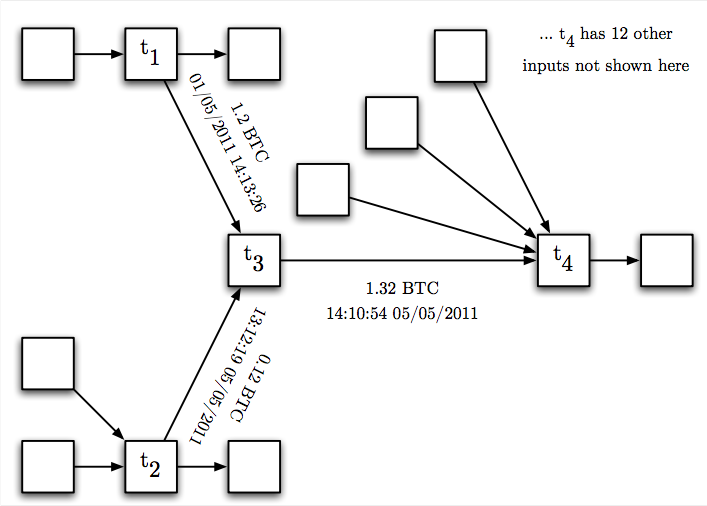
\includegraphics[scale=0.35]{images/transaction_graph.png}
% \caption{A sample transaction graph \protect\cite{ReidHarrigan13}.}
% \label{fig:transaction-graph}
% \end{center}
% \end{figure}

% \begin{figure}
% \begin{center}
% 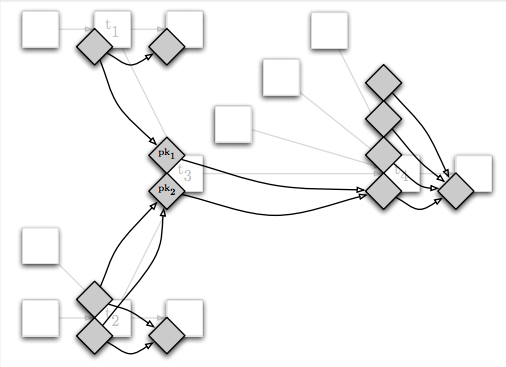
\includegraphics[scale=0.45]{images/transaction_user_graph.png}
% \caption{A sample user graph \protect\cite{ReidHarrigan13}.}
% \label{fig:user-graph}
% \end{center}
% \end{figure}

\subsection{Anonymization Attacks and Analysis Techniques} \label{sec:attacks}
%Current loss of privacy through voluntary identification/off network information, flow analysis, IP tracking. Needs more info

Intuitively, a successful attack on the anonymity of Bitcoin users yields a mapping between Bitcoin addresses, or public keys, to their respective owners. Depending on the success criteria for such an attack, the attacker may seek to find a single mapping for a particular user or a mapping for as many users as possible. Accordingly, there has been substantial research investigating the degree to which user anonymity is achieved \cite{ReidHarrigan13,BetterToBitter,Fistful12,Shamir13-bitcoingraph,Androulaki12-privacy}; proposed solutions presented in the literature are discussed in the following section.

\subsubsection{Network-Layer Attacks}
Although the original Bitcoin proposal suggests that anonymity, or rather pseudonominity, is possible due to the expected difficulty of associating Bitcoin addresses with their physical owners, there have been several works that disprove this claim. One of the earliest anonymity analyses was done in 2011 by Dan Kaminsky, a well-known security consultant and researcher. He assessed the anonymity properties of Bitcoin by performing the following experiment: First, he opened up a direct P2P connection to a large set of peers in the Bitcoin network. Under the assumption that the first appearance of a transaction stems from the original sender (unless an anonymizing layer such as Tor is used to obscure the source), it became fairly easy to combine the peer connections with some elementary traffic analysis to derive a mapping between Bitcoin addresses and IP-layer addresses \cite{kaminsky}. While IPs are rarely static due to DHCP-based IP address acquisition and the increasing ubiquity of mobile devices, it is not a significant leap to suspect that such knowledge could reveal the underlying user's identity, especially if offline auxiliary information is used (e.g., if the attacker is able to correlate the IP addresses to users using public forums or other applications). With this observation, a more active deanonymization attack, as carried out by Kaminsky \cite{kaminsky,ReidHarrigan13}, would involve malicious nodes scanning for Bitcoin clients listening to port TCP/8333 and opening a direct connection. While proxy services like Tor can hide outbound connections, an inbound connection will not be obfuscated. Again, by listening to transaction announcements over time, the client that first reports a transaction is the very likely one from whom it was initiated. This allows the malicious nodes to link transactions to IP addresses.

Using Tor enables one to obfuscate the source of a transaction. Unfortunately, it does not solve the problem entirely for several reasons. First, Tor does not provide perfect source secrecy. Tor is inherently susceptible to \emph{end-to-end correlation attacks} in which the attacker controls both ends of a Tor circuit used to send data (see Figure \ref{fig:tor-end-to-end}) \cite{tor-attack2}. Second, Tor was designed for low-latency, high throughput anonymous traffic. As such, it is susceptible to side channel timing attacks \cite{bitcoin-tor-wiki}. For this reason, the Chaum-like mixnets is often suggested but is not used in practice due to the lack of such services. 

\begin{figure}
\begin{center}
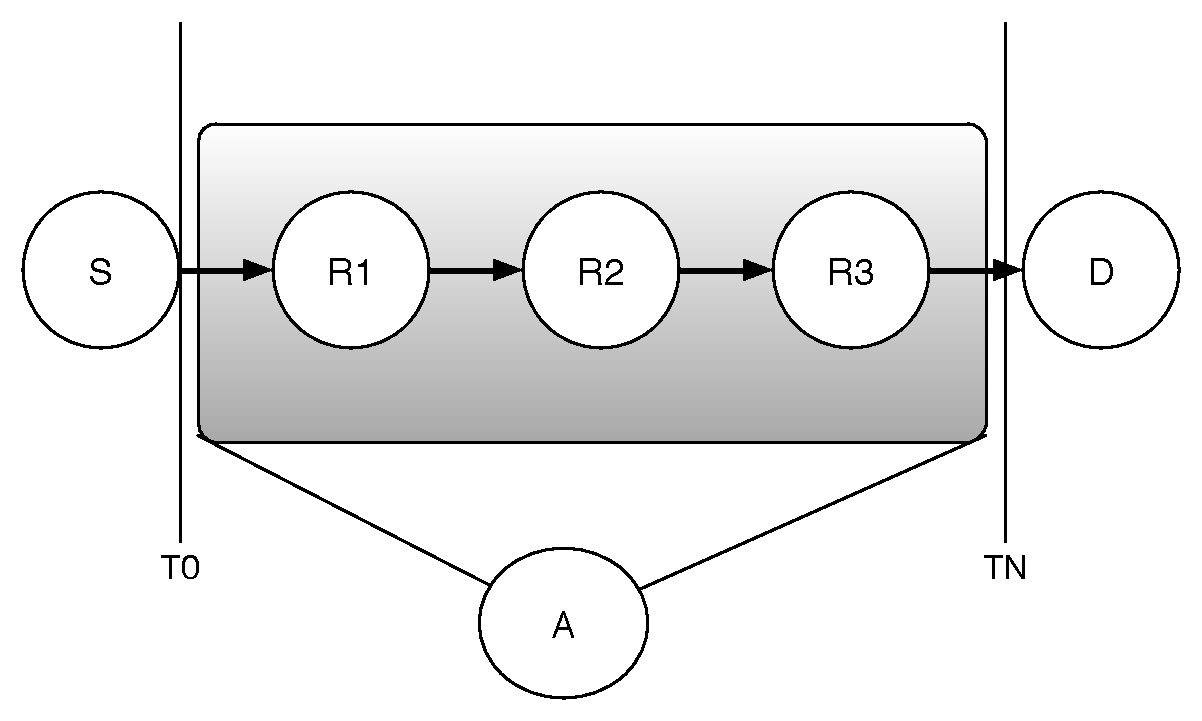
\includegraphics[scale=0.40]{images/tor_attack.pdf}
\caption{Illustration of an end-to-end correlation attack on Tor.}
\label{fig:tor-end-to-end}
\end{center}
\end{figure}

\subsubsection{Protocol-Layer Attacks}
Trivial attacks on anonymity involve using the Bitcoin block chain to follow all the transactions associated with that address. As users commonly have many addresses, a more sophisticated attack requires the adversary to link the known address with other hidden addresses and then analyze the transactions associated with those addresses. The two major heuristics for linking addresses are \emph{multi-address transactions} and \emph{shadow or change addresses}. Multi-address transactions are transactions with more than one source. Currently, Bitcoin allows for users to use more than one source address in a transaction, but does not allow multiple users to pay for one transaction. For example, suppose a single user owns two addresses, $\mathsf{addr}_A$ and $\mathsf{addr}_B$, and wishes to make a payment to another user via address $\mathsf{addr}_C$. Also suppose that $\mathsf{addr}_A$ has 3 Bitcoins (BTC) and $\mathsf{addr}_B$ has 2 BTC. The user uses both addresses to pay 4 BTC to $\mathsf{addr}_C$ and puts the remainder of 1 BTC to $\mathsf{addr}_D$. Since only one user can be the input to any transaction, anyone can deduce that $\mathsf{addr}_A$ and $\mathsf{addr}_B$ belong to the same user. \emph{Shadow addresses} or \emph{change accounts} are accounts created for change from a transaction. In the transaction above, $\mathsf{addr}_D$ is the shadow account that belongs to the same user that controls $\mathsf{addr}_A$ and $\mathsf{addr}_B$. Although not directly related to the Bitcoin system, the way Bitcoin clients handle shadow accounts can break address indistinguishability [4]. However, because shadow accounts rely on user behavior instead of an inherent property of the Bitcoin system, the shadow account heuristic is not as robust \cite{Fistful12}. Using these two heuristics, researchers have been able cluster addresses using the transaction graph \cite{Shamir13-bitcoingraph,ReidHarrigan13,Fistful12}. In any node where the user has revealed ownership of an address, the user's anonymity is lost.

Motivated by this observation, and relying on the accessibility of publicly accessible offline information relating to the Bitcoin system, Reid and Harrigen \cite{ReidHarrigan13} followed up on Kaminsky's work with an analysis of Bitcoin anonymity. To do so, they constructed the Bitcoin transaction and user graphs (see Section \ref{sec:vectors}) as an alternative representation of the flow of information in Bitcoin, and used \emph{passive} analysis techniques to derive user-to-address mappings. Such mappings were made by a combination of these dynamic graphs and offline auxiliary information acquired via other means. For instance, a store needs to have a publicly identifiable address in order to accept payment for goods or services. Users may also disclose address ownership when asking for donations or posting on Bitcoin forums \cite{Fistful12}. Large centralized Bitcoin services such as the Mt. Gox exchange service are also able to associate users with addresses as part of their service. Reid et al. also pointed out that by colluding the information of multiple accounts that participated in a transaction details about the owner can in fact be recovered. 

Shamir et al. \cite{Shamir13-bitcoingraph} also analyzed the transaction graph, deriving some global statistics, including an estimate that 78\% of the issued Bitcoins are not circulating, and an in depth analysis of a highly active region in the transaction graph. Their study was not focused on user anonymity, however. 

%%% EVALUATING USER PRIVACY PAPER
Recently, Androulaki et al. \cite{Androulaki12-privacy} studied the limits of user anonymity through the computational analysis of real-world and simulation-driven data. Their analysis was based on the assumption that users employ several standard practices for making transactions: multi-input transactions are allowed (although discouraged) and fresh shadow addresses are used to collect transaction change. The novelty in this study is the introduction of new quantifiable metrics by which user privacy and anonymity can be assessed. In particular, the notions of \emph{activity unlinkability} and \emph{profile indistinguishability} are defined, and metrics which can be used to measure the degree of unlinkability and indistinguishability are discussed. For completeness, we define these measurements and their metrics here.

Activity unlinkability is a general condition in which an adversary is not able to link two different addresses (address unlinkability) or transactions (transaction unlinkability) to the same user of her choice. It is clear that address unlinkability implies transaction unlinkability, as it is simple to link two transactions together if the addresses bound to these transactions are linked. Standard game-theoretic definitions of system-wide activity unlinkability are also given, which essentially state that an adversary cannot link two activities (addresses or transactions) with non-negligbly better probability than some adversary making uniformly random guesses of such links.

To quantify activity unlinkability by effectively measuring an adversary's success probability in this type of game, the authors propose the following technique: Let $\mathbf{E}$ and $\mathbf{GT}$ be  $n \times n$ matrices, where $n$ is the number of addresses in the system according to the transaction history. The $i,j$ entries of $\mathbf{E}$ are 1 if an adversary guesses that addresses $i$ and $j$ are owned by the same user, and $0$ otherwise. Similarly, the $i,j$ entries of $\mathbf{GT}$ are 1 if addresses are actually owned by the same user, and 0 otherwise. The error in an adversary's estimate for each address $i = 1,\dots,n$ is intuitively then the norm of the vector $\mathbf{E}[i,*] - \mathbf{GT}[i,*]$ (i.e., the difference between the guess and the real value), and the maximum error in this estimate, which is analogous to an upper bound on the probability of the adversary's success in the activity unlinkability game, is then the maximum error over all addresses. For the ``random guess'' adversary, $\mathbf{E}$ is constructed such that each $\mathbf{E}[i,j] = \pi_{i,j}$ if there is some external knowledge available to this attacker and $\pi_{i,j}$ represents the probability, or confidence, based on this apriori knowledge, and $\mathbf{E}[i,j] = \rho + (1 - \rho)/2$ otherwise, where $\rho$ is the fraction of addresses in the transaction history that cannot possibly be linked to multiple users. The latter scenario occurs when the address is owned by some user who only has one address. Given these definitions, the overall advantage of an adversary in this activity linkability game is then the difference of the two error estimates. 

Profile indistinguishability is a condition in which an adversary is not able to reconstruct the profiles (collection of representative addresses or transactions) of \emph{all users} who participated at some point in the block chain. The fact that all profile indistinguishability holds if and only if the adversary cannot reveal profiles for all users makes it an intuitively stronger notion of privacy than address unlinkability, which only requires some information linkage with respect to a single user. Analogous to the above definition, a system deployment is said to enjoy profile indistinguishability if the global transaction history does not provide any non-negligible advantage in deriving the correct (address or transaction) profiles when also given the total number of users in the system. 

The metrics used to quantify profile indistinguishability are related to those used to quantify address unlinkability, though somewhat more contrived. In particular, they are based on the definition of some similarity function $\mathsf{Sim}$, which takes as input the adversary's estimate of the user profiles, $\mathbf{E}_\mathsf{prof}$, and the actual user profiles $\mathbf{GT}_\mathsf{prof}$. If we define the output of this function given inputs $\mathbf{E}_\mathsf{prof}$ and $\mathbf{GT}_\mathsf{prof}$ as $\mathsf{Sim}(\mathbf{E}_\mathsf{prof}, \mathbf{GT}_\mathsf{prof})$, then the advantage of an adversary in the profile indistinguishability game is simply $\mathsf{Sim}(\mathbf{E}_\mathsf{prof}, \mathbf{GT}_\mathsf{prof}) - \mathsf{Sim}(\mathbf{E}_\mathsf{prof}^R, \mathbf{GT}_\mathsf{prof})$ (where the second term denotes the estimate made by a ``random guess'' adversary). Computing $\mathsf{Sim}$ relies on \emph{normalized mutual information} (NMI) and \emph{adjusted mutual information} (AMI). According to \cite{privacy-19,privacy-20}, NMI increases in magnitude as the similarity of the two input profile groupings increases. Conversely, AMI decreases in magnitude (towards 0) as the input of the adversary's guessed profile grouping appears to be uniformly random (i.e., it is highly similar to a random grouping). Details of these computations are omitted for brevity. 

Given these privacy measurements and supporting metrics, the authors then quantitatively assessed user privacy in a simulation of Bitcoin transactions in a university setting. This experiment used the simulator to gather the ``ground truth'' information about users and their addresses in a system, performed various machine learning behavior-based analysis techniques such as k-means clustering (KMC) and Hierarchichal Agglomerative Clustering (HAC) to formulate an adversary's guess in deanonymizing clients, and then calculated the resulting success (adversarial advantage) in the address unlinkability and profile indistinguishability games. The interesting results for these calculations after varying the fraction of ``privacy-aware'' users, i.e., those that avoid multi-input transactions and use fresh shadow addresses, and the total number of users in the simulation are shown in Table \ref{tab:eval-privacy-results}. Observe that in nearly all cases the adversary has a clearly non-negligible advantage when given some apriori knowledge about the users in the network. These results highlight the extent to which anonymity is not upheld in Bitcoin.

\begin{table*}
\begin{center}
\caption{Adversarial advantage when given partial knowledge of users in the (simulated) Bitcoin network.}
\label{tab:eval-privacy-results}
    \begin{tabular}{|l||ccccc|}\hline
    ~                   & 100 (50\%) & 200 (0\%) & 200 (50\%) & 200 (100\%) & 400 (50\%) \\ \hline
    $\mathbf{Link}_A$   & $0.91 \pm 0.01$ & $0.90 \pm 0.01$ & $0.91 \pm 0.01$ & $0.92 \pm 0.01$ & $0.93 \pm 0.01$ \\
    $\mathbf{Prof}_A^a$ & $0.76 \pm 0.01$ & $0.87 \pm 0.01$ & $0.79 \pm 0.01$ & $0.70 \pm 0.01$ & $0.80 \pm 0.01$ \\ \hline
    \end{tabular}
\end{center}
\end{table*}

% \todo[inline]{On Bitcoins and Red Balloons - fix this summary}
% The peer-to-peer design of the Bitcoin system relies on information sharing.  However, because confirming transactions has a monetary reward, it is not in a node’s interest to share information about transactions.  A possible solution is to introduce a referral reward for all the nodes that notified the node which confirmed the transaction.  This solution introduces the problem of Sybil attacks where a node will create clones in order to receive the reward for the both the confirmation and the referral.  The solution is to create a situation where it is most rewarding for a node to share information and never to clone itself.  Let the node which announces the transaction be the root of a directed graph.  The graph is a directed graph as knowledge of the transaction only flows one way from the root.  Let the node which confirms the transaction, v, be a distance h away from the root.  In order to facilitate sharing, every node on the path from the root to v is given a reward of B.  However, if h is greater than H, an arbitrary distance, then no node is awarded any reward.  If h is less than H, then v receives a reward of 1+B*(H-h+).  This is to mimic the reward v would have gotten if it duplicated itself H-h times.  If external competition is low, nodes would prefer to clone themselves in order to receive the maximum payout.  However, if knowledge of the transaction is high, a node would prefer not to clone itself to increase the chance of being in the reward chain.  With a sufficiently high number of seeds and a reward value relative to 1/H, the system encourages information transfer without cloning or Sybil attacks.

\section{Proposed Solutions} \label{sec:solutions}
Generally speaking, solutions to address the anonymity issues in Bitcoin roughly fall into one of the following three categories:
\begin{enumerate}
	\item Use an anonymity layer to obfsucate the source IP address of Bitcoin users,
	\item Use mixing services to unlink transactions from their owners, and
	\item Modify the Bitcoin protocol using cryptographic techniques that improve guarantees of anonymity.
\end{enumerate}

\subsection{Anonymity Layers}

The basic design and use of mix networks is credited to Chaum and dates back to more than three decades \cite{Chaum81-Mix}. The essential idea of a mix network is illustrated in Figure \ref{fig:mix-design}. Senders wrap their message in layers of encryption using the public keys of randomly selected mixing service nodes (mix node), who then receive a set of encrypted messages, decrypt and shuffle the messages, and then send them to another mix node or the intended recipient. Clearly, the role of each mix node is to hide the source of original messages by obfuscating their flow through the network. To initiate an untraceable message (email) in the original design, which was intended to be used for untraceable email, Alice encrypts a message to Bob with Bob’s public key, appends Bob’s address, and then encrypts the entire message with the mix server’s public key. The mix server receives the message, decrypts it with the mix server’s private key, and then sends the message to Bob after waiting some non-deterministic amount of time. The order of outgoing messages is hidden by the fact that the mix server receives messages that are uniformly sized and rearranges them in lexicographical order.  Bob receives the message from the mix server and decrypts it with his private key.

A ``cascade'' or series of mixes (see Figure \ref{fig:mix-design}) can increase the secrecy of the messages as all of them must be compromised before a message can be traced.  The protocol is similar to a single mix with the exception that messages are encrypted with all the mix server’s private keys.

Since mixnet services are not generally available, Bitcoin users are often suggested to use Tor \cite{tor} to achieve similar anonymity properties with strong (but not perfect) protection against eavesdropping and traffic analysis attacks. To use Tor with Bitcoin, a separate software client must be installed which establishes circuits from a pool of anonymizing routers through which all Bitcoin traffic can flow. To redirect this traffic, the user's Bitcoin client must be configured to send all traffic through the local Tor proxy using the SOCKS protocol (i.e., 127.0.0.1:9050, where 9050 is the default Tor port number). Despite the popularity of Tor as a network anonymity layer, it is intended for low-latency, high-throughput traffic that is susceptible to targeted attacks by active adversaries \cite{tor-attack1,tor-attack2}.  

%%%%

%%% TODO: related work on mixing design and anonymity guarantees
% 17, 21, 10, 
% 17: Raymond, J.: Traffic analysis: protocols, attacks, design issues, and open problems. In: PET (2001)
% 21: Sako, K., Kilian, J.: Receipt-free mix-type voting scheme - a practical solution to the implementation of a voting booth. In: EUROCRYPT. pp. 393–403 (1995)
% 10: Golle, P.: Reputable mix networks. In: PET (2004)

\subsection{Coin Mixing Services}
Mixing services in the context of Bitcoin are distinct from traditional mixnets. In particular, mixers are used to anonymously collect or aggregate coins from clients, mix them internally (i.e., among several different Bitcoin addresses), and then redistribute coins back to the sources in equal denominations after some predefined amount of time. The role of a mixing service is illustrated in Figure \ref{fig:mix-bitcoin}. The obvious goal is to break, to the maximum extent possible, the link between the change address and signing address, thus improving the sender's overall anonymity. Also, it is important to emphasize the element of time with mixing services; contrary to anonymity layers like Tor, which were designed for low-latency, high throughput anonymous connections and are therefore susceptible to timing side channel attacks, mixing services that introduce a mandatory delay prohibit (to some degree) such attacks.

\begin{figure}
\begin{center}
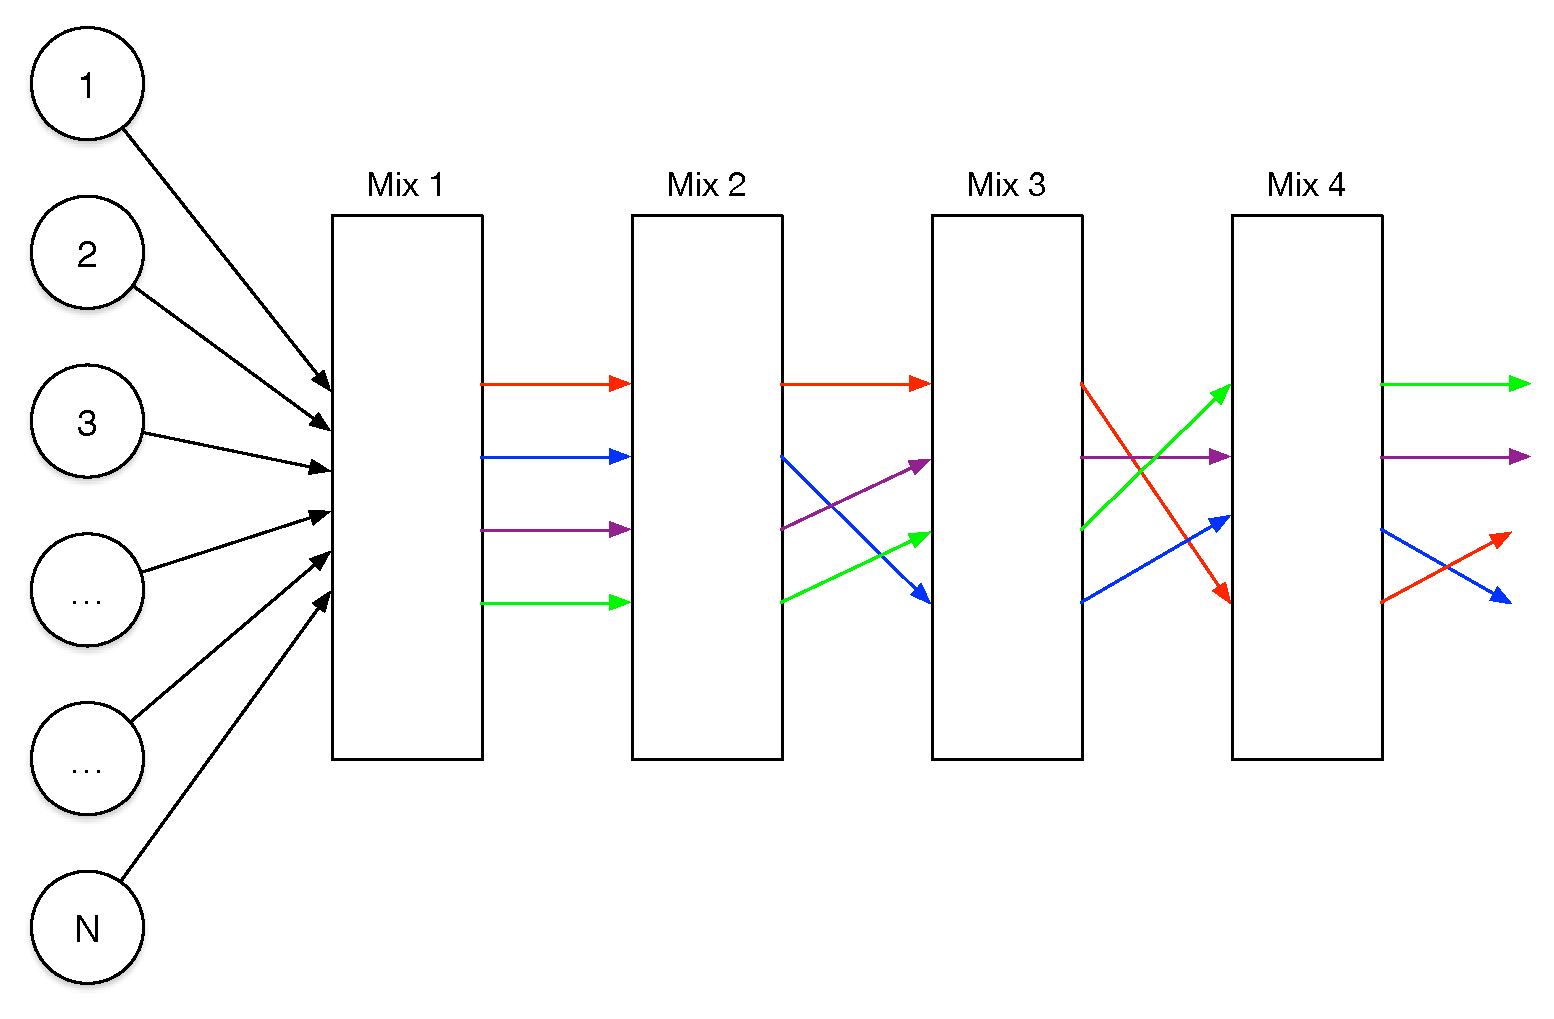
\includegraphics[scale=0.35]{images/mix_design.pdf}
\caption{Mixnet cascade.}
\label{fig:mix-design}
\end{center}
\end{figure}

\begin{figure}
\begin{center}
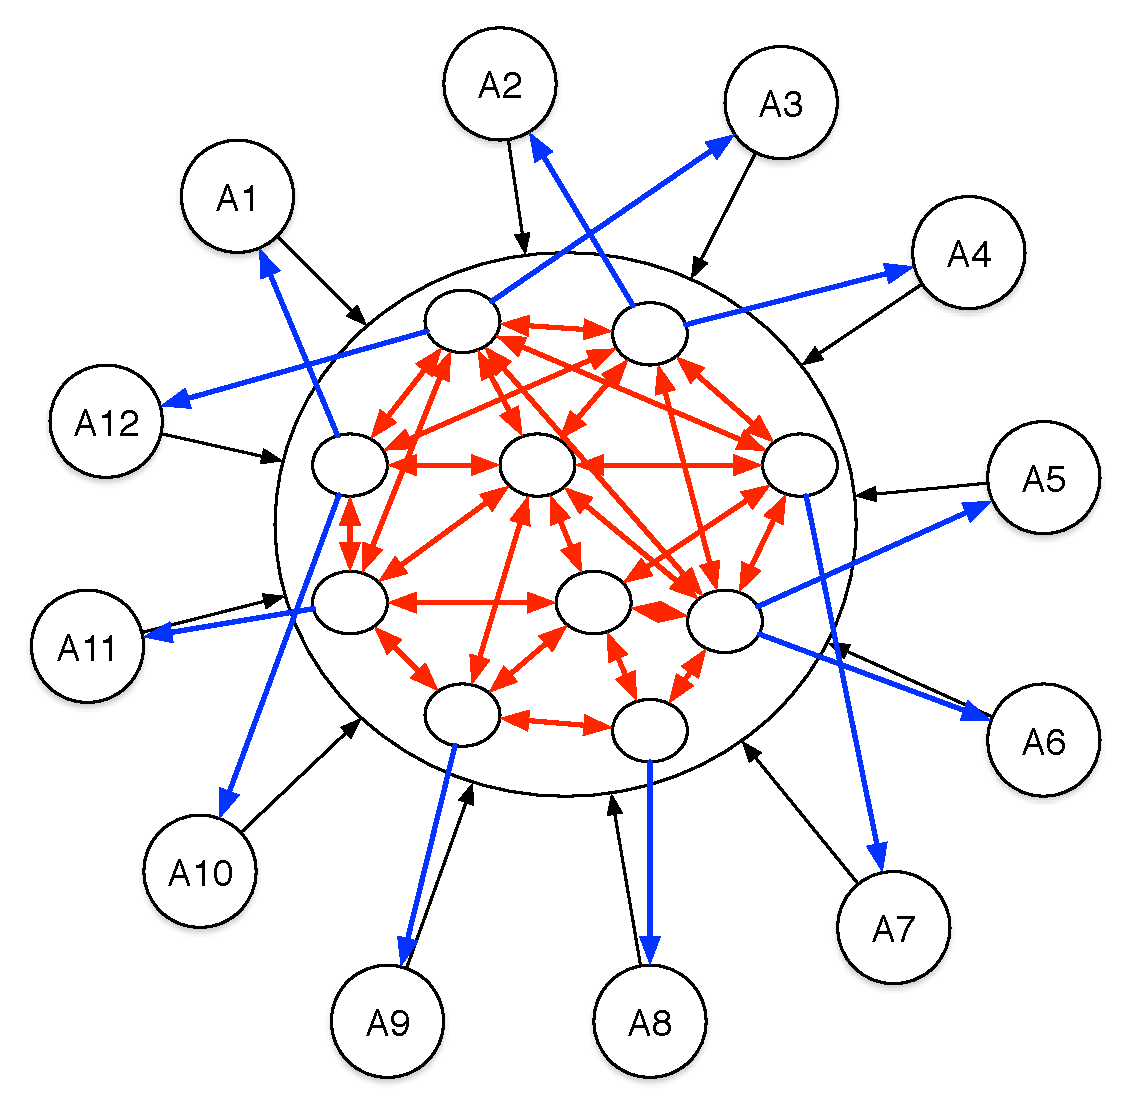
\includegraphics[scale=0.35]{images/mix_bitcoin.pdf}
\caption{Bitcoin fund mixing service node.}
\label{fig:mix-bitcoin}
\end{center}
\end{figure}

Unfortunately, Bitcoin mixing services naturally require a certain level of trust on behalf of the user. In particular, there is nothing in the current Bitcoin system that prevents a malicious mixing service from aggregating a large collection of coins and then abandoning their duty as a mixing service, thereby stealing all of its client's coins. Of course, such financial losses can be minimized if the user only sends funds to the mixing services in small amounts, but it does not eliminate the problem; users would then need to sequentially small small amounts to the mixer, thus drastically increasing the payout time. Therefore, we identify mixing \emph{theft} as a primary threat to users, as well as deanonymization, since the mixing service naturally learns the client's input transaction-signing and output change address.

Given these problems with simple mixing services in the context of Bitcoin, there has been several attempts to modify their deployment and usage in order to avoid the aforementioned threats. One work by Barber et al. \cite{BetterToBitter} explored such a modification under the assumption that there does not exist an underlying trust architecture that can be relied upon to prevent the attacks; their conclusion was that the only feasible alternative is to use a \emph{fair exchange protocol} between the users and mixing service to ensure that all input coins are eventually paid back. Unfortunately, their proposed protocol must be integrated with the existing Bitcoin protocol - it is not natively supported. For completeness, we highlight the main features of their approach here. The fair exchange protocol between a sender and mixing service, denoted as parties $A$ and $B$, respectively, requires three types of transactions:
\begin{enumerate}
	\item Commitment transactions to commit a party to a coin exchange.
	\item Refund transactions to refund a party's committed coins at a future date in case the other party aborts the protocol.
	\item Claim transactions to claim the other party's committed money. 
\end{enumerate}
After establishing a set of shared secrets using offline or online techniques akin to Diffie Hellman key exchange, $A$ and $B$ then begin the fair exchange protocol, which proceeds as follows:
\begin{enumerate}
	\item $B$ generates a committment and refund transaction, with the help of $A$, and broadcasts both transactions. The committment transaction is constructed such that its respective funds can be redeemed using either the corresponding refund transaction (after the protocol ``times out'', or one party fails to complete their duties within a pre-defined ) or a to-be-generated claim transaction. \footnote{The refund transactions are constructed with the output coins being redirected back to their original owner so that the coins are not lost in the event that the protocol does not complete.}
	\item Simultaneously, $A$ generates a committment and refund transaction, also with the help of $B$, and broadcasts both to the network. 
	\item After both parties are committed to the exchange, they must claim their coins. In order to do so fairly, $B$ first claims $A$'s coins using $A$'s refund transaction, and by doing so, enables $A$ to claim $B$'s coins through $B$'s refund transaction. This refund process works as follows: $B$ modifies the output of $A$'s refund script (a part of the transaction block) to be redirected to $B$'s recently generated address, and also modifies the input of the script to reveal the ``secret'' values that enables $A$ to modify her refund transcation. Once $B$ publishes his claim transaction, thus taking $A$'s funds, $A$ can then receive the secret values from $B$'s claim transaction to modify $B$'s refund transaction output to point to her own recently generated address. $A$ then broadcasts her claim transaction to claim $B$'s coins, thus completing the exchange.
\end{enumerate}
Note that if a protocol ``timeout'' occurs, then the refund transactions were never properly modified by both parties to steal the other party's coins, and no exchange took place. 

With an existing public key infrastructure and means to securely transfer the secrets used in the transaction generation, this protocol will prevent malicious mixing services from stealing user's coins. However, it requires modifications to the underlying Bitcoin protocol that aren't readily supported. Most importantly, it requires that transactions support the notion of timelock (i.e., points in time when they can no longer be changed). 

%%% MIXCOIN
Motivated by the desire to achieve the same level of trust without modifying the underlying Bitcoin protocol, Bonneau et el. \cite{mixcoin} recently proposed Mixcoin, a natively-supported protocol for building accountability into mixing services. The principal idea used to achieve mixing accountability is to rely on simple economics, rather than cryptographic solutions, to ensure that mixing services will benefit more from honest participation in mixing rather than from theft. Properly aligned financial incentives ensure that theft is not likely to happen, else the mixing service's reputation is permanently destoryed. However, as the authors note, there is no (protocol-level) mechanism that can be used to gaurantee that a mixing service is not linking client input and output addresses; software implementations of mixing services may purposefully or accidentally store this information and thus render it susceptible to exposure if compromised. Such means of acquiring auxiliary information are outside the scope of this survey and we do not discuss them further.

The key insight to achieving business-incentivized accountability through financial incentives is that mixing nodes will provide warranties stating that they claim to complete a mixing operation prior to some agreed-upon deadline. If the mixing node operates dishonestly or steals the client's funds, the client then simply broadcasts the warranty to the network, which is signed by the mixing node using a long-term private key, which can then be verified by all nodes in the network using the corresponding public key. The net effect is that no more (intelligent) clients will do business with the mixing node. With an appropriate fee selection it is therefore economically sensible to behave honestly rather than attempt to steal funds since mixing nodes are paid for their efforts by means of a mixing fee.

The fundamental protocol used to achieve this accountability operates as follows:
\begin{enumerate}
	\item A client $A$ generates a tuple $T = (v, \mathsf{addr}_{\mathsf{in}}, \mathsf{addr}_{\mathsf{out}}, t_1, n)$, where $v$ is the BTC amount to send, $t_1$ is a time by which $A$ will transfer the $v$ funds, and $n$ is a random nonce. This tuple is then sent to the mixing node $M$.
	\item If $M$ accepts the parameters, a fresh escrow address $\mathsf{addr}_{\mathsf{escrow}}$ is generated at which the funds can be acquired by $M$, a deadline $t_2$ by which the funds will be transferred, and a mixing fee rate $p$. These parameters are then signed using the long-term key $K_M$ to generate a warranty, and both are then sent to $A$.
	\item If $A$ accepts $t_2$ and $p$, $A$ transfers the funds to $\mathsf{addr}_{\mathsf{escrow}}$.
	\item After receipt of the funds at $\mathsf{addr}_{\mathsf{escrow}}$, $M$ will return the same amount of funds, minus the agreed-upon transaction fee, to $\mathsf{addr}_{\mathsf{out}}$.
	\item Both parties delete the parameters used in the transaction.
\end{enumerate}

Observe that $A$ may choose to opt out of the protocol at any point prior to the transfer of the funds by $A$. If $M$ does not act honestly, $A$ simply broadcasts the signed warranty to other nodes so that they may see $A$ was cheated. It is also important to note that, just as in traditional mixing schemes, these mixing nodes may be used sequentially to increase anonymity through multiple mixing rounds. This is done by using the output address of the $i$-th round of mixing as the input address of the $(i+1)$-th round, thereby creating a chain through which the client's funds flow through potentially separate mixes. 

While simple, there are several underlying issues that must be addressed in practice to ensure anonymity:
\begin{itemize}
	\item All Bitcoin chunk sizes should be uniform.
	\item The mixing service should choose escrow addresses at random when transferring funds from a client's input address to their specified output address.
	\item Transaction fees should be randomized (from an appropriate source of randomness, such as a Beacon \cite{nist-beacon} or some PRG computed based on the transaction block chain).
	\item There should never be two outstanding warranties for the same input address issues at the same time.
	\item Clients should not publicize their freshly created input addresses until mixing has initiated, else a malicious party could perform a DoS attack (due to the above requirement) by requesting a warranty for some observed or predicted input address.
	\item Clients should use separate mixes when aggregating their mixed funds to make a transaction, or else their anonymity set reduces to the intersection of the anonymity set for each of the mixed funds.
\end{itemize}

A brief analysis of the anonymity properties provided by Mixcoin was also presented. Of the most trivial observations are that mixing message replay is impossible due to the single-warranty issuance property stated above, and also that blocking client-to-mix or mix-to-client transactions are not feasible under the standard assumption that the majority of Bitcoin users and miners are not malicious. They also derived a value for the maximum mix delay $\delta_{max}$ (i.e., the time between receiving input funds and transferring output funds) to optimize the client's anonymity set. If a mix receives input transactions at a stable rate where $Q$ chunks are mixed in a single round (i.e., the total number of funds mixed is equal to $Q \times v$, where $v$ is the baseline uniform mixing input), then the anonymity set of each client is roughly $Q(\delta_{max} - w + 1)$, since fresh input and output keys are used for each of the $Q$ chunks for a particular user, and where $w$ is the minimum difference between $t_2$ and $t_1$ (observe that the final mix delay, uniformly generated, thus falls in the interval $[w, \delta_{max}]$). For $98 \leq Q \leq 4096$, it was found that $\delta_{max} = 7$ since the anonymity set grows by 
\begin{align*}
1 + \frac{\log_2Q(\delta_{max} - w + 1)}{1 + w + \frac{\delta_{max} - w}{2}}.
\end{align*} 

It should also be clear that the anonymity set of a particular chunk \emph{is not} the size of the fund chunks in the mixing node. Rather, it is the size of the set of fund chunks that were mixed at the same time, i.e., those which overlap in the same round within the mixing service. For this reason, longer mixing delays or multiple mixing nodes in sequence benefit all mixing participants, and it is conjectured that these delays will converge to reasonably steady values in practice. Simulations performed by the authors showed that as the number of overlapping mixing rounds for a set of $m$ mixes increases, where each round transfers $Q$ chunks, the statistical distance between the PDF of the anonymity set of each chunk rapidly approaches the uniform distribution. Put simply, this means that out of all $Qr$ chunks (where $r$ is the number of rounds), the probability that an adversary can correctly associate a chunk with its input client is roughly $(Qr)^{-1}$.

% \begin{figure}
% \begin{center}
% 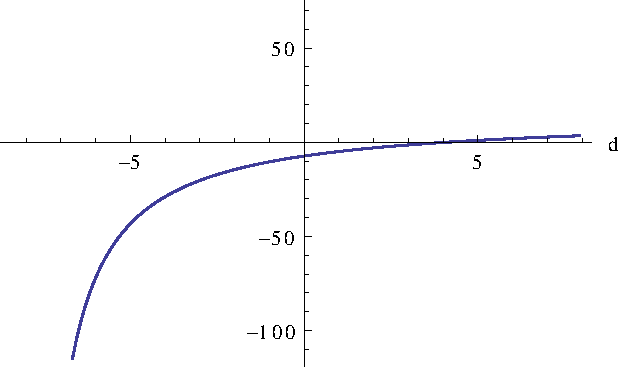
\includegraphics[scale=0.75]{images/mixcoin-delay_plot.pdf}
% \label{TODO.}
% \label{fig:mix-design}
% \end{center}
% \end{figure}

%% TODO: mixcoin section 5.4 finish up
There is one more subtle yet important issue concerning the use of these mixing services. Recall that the input from one client $A_1$ may be used to provide output funds for another client $A_2$, and each of these inputs are associated with their providers, $A_2$ will learn that $A_1$ has interacted with the mixing service. Therefore, to deanonymize clients, an active adversary can request the mixing of many funds in hopes of probabilistically determining whether or not a particular user $A$ has used a mixing service. This type of deanonymization attack is probabilistic because the input provided by $A$ is only routed to the adversary's output according according to some probability distribution. Fortunately, since each use of the mixing service costs a certain fee, an attacker will, on average, have to invest a great deal of funds in hopes of learning whether or not $A$ has interacted with the mixing service. Therefore, as previously mentioned, clients should use separate mixes whenever possible if their mixed funds (chunks) are to be used together in a single transaction. Beyond the immediate fact that her anonymity set reduces to the intersection of the anonymity set for each mixed chunk, it also reduces the likelihood that compromised or malicious mixes can deanonymize the client. 

\begin{figure}
\begin{center}
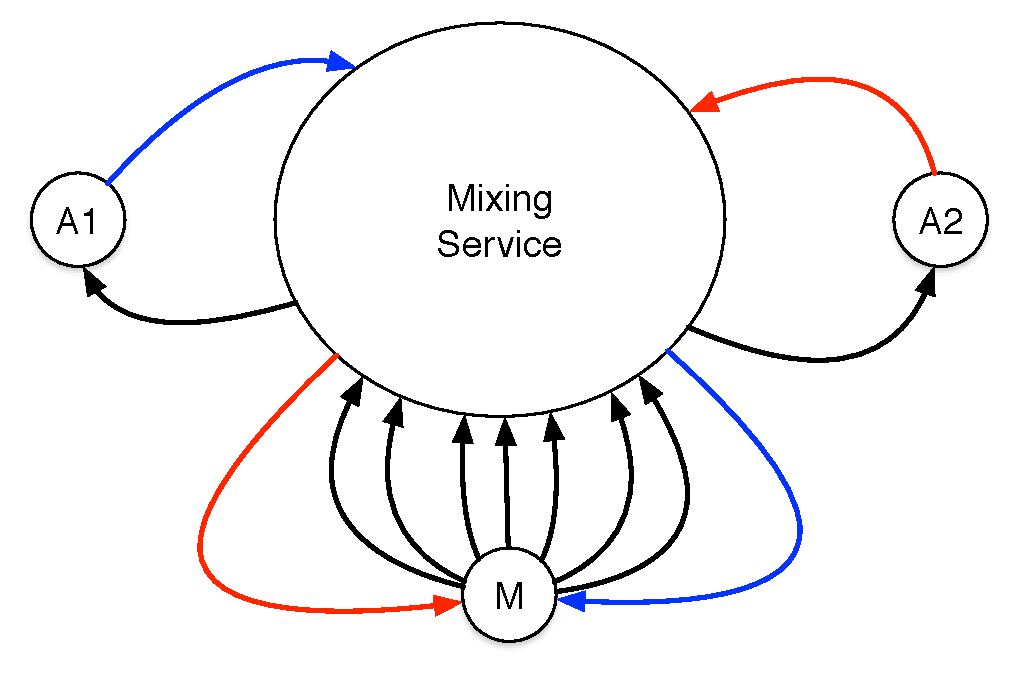
\includegraphics[scale=0.45]{images/mixcoin_deanon.pdf}
\caption{Visual depiction of an active deanonymization attack in Mixcoin.}
\label{fig:mix-design}
\end{center}
\end{figure}

Finally, we note that there are several protocol-level side channel attacks that can be leveraged by an adversary to decrease a client's anonymity, as follows:
\begin{itemize}
	\item Passive observance of a client requesting a certain amount of mixed funds and then witnessing that same amount appear in a single transaction in the future effectively provides a probabilistic link from the later transaction to the observed client.
	\item Bitcoin transactions (and therefore, mixed funds) are timestamped, and the provenance information of transaction block chains can therefore be used to link clients to future transactions if both the client who originally owned the unmixed funds and the time at which those funds were mixed is known. This can be avoided by paying with funds that were mixed at the same time, paying to re-mix all chunks every time a payment is to be made, and time-delayed continual mixing, among other possibilities. Observe that the client will incur additional mixing costs for the latter two solutions, which may or may not be acceptable given the level of anonymity desired, and so the client will have to intelligently choose when to mix funds at her own discretion.
\end{itemize}

%%% COINJOIN
CoinJoin \cite{coinjoin} is another method inspired by mixing services to support multi-user inputs in a Bitcoin transaction without sacrificing user anonymity. In CoinJoin, users agree on a common output size and then combine all their transactions of that size into one big transaction. The aim of this method is to obfuscate which user is the input to an output and prevent the association of multiple addresses in a transaction to one user. It is not clear which user is associated to a certain output if multiple transactions with the same sized output are combined together; any user could have paid for any output. For instance, if Alice has a 1 Bitcoin transaction to Carol and Bob has a 1 Bitcoin transaction to Dave, they can combine their transactions together to create one transaction with two outputs for 1 Bitcoin each. Now it is unclear if Alice paid Carol or Dave. With more simultaneous users, the ability to accurately track transactions would decrease proportionally.

CoinJoin allows for multiple inputs per user and combines them all into one transaction. With enough users, the transaction would hide which of the many accounts belong to which user. Although some analysis can be done on the inputs and outputs, it would not have nearly the same accuracy as the current heuristic of one user per transaction.

The simplest implementation of CoinJoin can be done with a ``meet-up'' server to coordinate transactions. A decentralized version can be used, but the issues with coordinating transactions cause complexity.

The most notable feature of CoinJoin, aside from increased anonymity, is that it works \emph{without} any modification to the Bitocoin protocol, which is untrue for solutions like the fair-exchange mixing service and Zerocoin (see the following section). The transactions from CoinJoin are identical to normal Bitcoin transactions. A potential development involves moving away from a centralized server that knows all the mappings to one that doesn't and eventually a decentralized system. It is also unknown how many sessions does the protection of privacy extends. Finally, similar to other financial systems, CoinJoin does not hide the user's IP address; an anonymity layer such as Tor is needed to obfuscate this information from a sender's peers.

\subsection{Cryptographically Enhanced Anonymization Techniques}
We now describe solutions that build upon the Bitcoin protocol to improve sender anonymity. To our knowledge, the earliest such attempt (which is actually quite recent) is Zerocoin, a distributed, anonymous cryptocurrency using Bitcoin as a form of backing currency. At a high level, the underlying idea behind the Zerocoin protocol is amazingly simple and intuitive, and it stems from the fact that Bitcoin transactions are publicly linked together and therefore susceptible to passive network analysis techniques (as previously discussed above). Zerocoin breaks the links between transactions using cryptographic techniques that yield the same property of Bitcoin transaction chains (namely, the flow of coins and current value of a transaction). Ultimately, Zerocoins are not identified by public keys as in the case of the backing Bitcoin currency; rather, they are identified by a commitment $C$ to randomly generated secrets (i.e., a serial number $S$ associated with the coin and ``opening value'' $r$) only maintained by the owner of the coins. To do this, Zerocoin leverages cryptographic accumulators, or primitives that enable a party to sign a collection of objects as opposed to a single object and accumulate the result into a single signature digest (in this case, the collection would be the set of previous transactions), and zero-knowledge proofs. 

The use of these cryptographic primitives as follows. Whenever a user wants to spend Zerocoins they receive associated with some committment $C$, the owner must reveal $S$ publicly and then provide a proof that they are also in possession of $r$ capable of opening some commitment $C_i \in \{C_0,\dots,C_{n-1}\}$, the set of all committments made in the system. The owner uses $r$ to generate a (zero-knowledge) ``signature of knowledge'' $\pi$ that is equivalent to stating that the owner can open some committment (coin) $C_i \in \{C_0,\dots,C_{n-1}\}$, without revealing which coin they actually own (hence, the signature of knowledge is actually a zero-knowledge proof). Technically, to generate this proof, the owner accumulates the results of all coins used to finance the transaction into an RSA-based accumulator, produces an accumulator witness $w$ (the accumulated total of all bitcoins in the transaction minus the value of the Zerocoins to be spent), and finally, generates $\pi$ that enables other entities to \emph{publicly} verify that the value in the accumulator was generated by the entity who derived this proof and was in possession of the Zerocoins coins (committments) necessary to fund this transaction. Zerocoin peers can then verify an accumulated value, representing virtually the same information as a Bitcoin transaction graph, using $\pi$.

From an anonymity perspective, Zerocoin ensures that given two Zerocoins and one ``spend'' coin, one is not able to determine, using publicly available knowledge, which coin was spent (i.e., the adversary's advantage in correctly identifying the spent coin is negligible in the security parameter of the system). However, in practice, Zerocoin is inherently limited in that the size of the spender anonymity set can be significaly reduced under certain circumstances. For example, if a user mints and subsequently spends $5$ Zerocoins, it is clear to an adversary participating in the system that all $5$ coins were spent since they can simply verify the transactions; the adversary does not, however, know which coin was spent in which transaction, implying that the anonymity set cardinality is $5$. Now, if the same user not mints and spends another coin, one would hope that the anonymity set would increase to $6$. Clearly, this is not the case, as the attacker can easily deduce that the last minted coin was spent in the last transaction, and thus the cardinality of the anonymity set is exactly $1$. Based on this observation, the anonymity set cardinality for a single coin is clearly bounded below by the number of coins minted between the time of the candidate coin's mint and spend, and upper bounded by the total number of minted coins in the system. Other anonymity issues of Zerocoin relate to the fact that all minted and spent coins are public knowledge, and that all transaction denominations are also publicly available. These can easily be addressed in practice, however.

The mathematical details of accumulation and witness verification are out of the scope of this survey. However, we note that security of both schemes relies on the hardness of the Strong RSA and Discrete Logarithm assumptions. As such, the operations required for accumulation and verification come at the cost of additional computational overhead. Furthermore, Zerocoin requires a preliminary, potentially offline, setup phase in which the parameters for the accumulator and zero-knowledge scheme. Aware of these pitfalls, the authors propose a variety of optimizations for improving Zerocoin performance. Namely, they introduce the notion of accumulator checkpoints, which are essentially timestamps that capture the value of an accumulator after each transaction in a recently mined block, thus removing the need for a verifier to re-compute the entire accumulator value from scratch upon every invocation. 

Secondly, the authors discuss methods in which the zero-knowledge proof scheme can be improved. Their preliminary experiments revealed that the size of proofs often exceeded the MTU of Bitcoin transactions, which prohibits its immediate use since Zerocoin relies on Bitcoin for the backing source of Zerocoin funds (i.e., Bitcoins are used to mint Zerocoins) and transaction block graphs to timestamp the state of the system. Rather than modify this MTU limitation so that proofs can be stored alongside accumulator checkpoints in the transaction block chain, the authors propose to store and access proofs using a distributed hash table or non block-chained storage mechanism in Bitcoin. With respect to the computational cost of proofs, the authors propose a distribtued verification strategy so as to not make every node verify the proof of every new transaction block. Doing so would be a large computational burden on verifiers, which should be quick, as opposed to miners, whose efforts are justified via transaction fees. Internally, the chosen zero-knowledge signature of knowledge scheme consists of $n$ repetitions of the same proof to reduce the probability of forgery to $\mathcal{O}(2^{-n})$, and so by requiring that each node \emph{randomly} selecting a subset of these $n$ proofs to compute and it is possible to achieve the same proof security guarantee with a significantly reduced amount of duplicated effort.

%%% Pinocchio Coin
Pinocchio Coin \cite{pinocchio} is a very new attempt to optimize the Zerocoin protocol. Whereas Zerocoin uses an accumulator based on the Strong RSA assumption and proofs founded on double discrete logarithms, Pinocchio Coin uses elliptic curves and bilinear pairings to achieve virtually the same behavior with significantly less overhead. As such, Pinocchio Coin follows the same process as Zerocoin for the setup, mint, spend, and verify protocols: The setup phase involves creating a suitable pairing-friendly elliptic curve in the security parameter and then configuring the parameters for the Pinocchio proof system. As previously stated, minting, spending, and verification are analogous to the Zerocoin protocol with the exception that proofs are generated without the need to accumulate past commitments (though the proof generation still requires all commitments $C_0,\dots,C_{n-1}$ as input to ensure correctness). 

The Pinocchio proof of work was originally designed as a generic proof of work to be used in applications such as cloud computing. The system takes a set of operations and converts them into proof of work that can be seen as a zero knowledge proof. The primary advantage of using Pinocchio Coin over Zerocoin is that the size of each proof is significantly smaller; Pinocchio proofs are less than 400 bytes as opposed to Zerocoin's 50kB proofs, which are well within the Bitcoin MTU limit. One potential disadvantage of using Pinocchio Coin is that there is no security analysis as of yet \cite{pinocchio}. Futhermore, although Pinocchio serves as an efficient general proof compiler, it is unknown whether or not specialized systems such as ZKPDL \cite{zkpdl}, a general zero-knowledge proof system intended to be used with e-cash technologies, would exhibit better performance in the Zerocoin framework.

%%%%%%%%%%%%%%%%%%%%%%%%%%%%%%%%%%%%%%%%%%%%%%%%%%%%%%%%%%%%

%Centralized mixes similar to Chaums anonymous email (BitFog, BitLaundry, Blockchain.info) and decentralized mixes (Zerocoin).

% The anonymity problem in Bitcoin was later addressed by ZeroCoin [13] which allows the implementation of a Zero- Knowledge based decentralized coin mixing service. Earlier Hanke et al. [10] presented a Pay-to-Contract Protocol that is built on top of Bitcoin and secures transactions between
% merchants and their clients. CommitCoin [6] is another system that builds on the blockchain to carbon date commitments.

%[5]Dorit Ron and Adi Shamir. Quantitative Analysis of the Full Bitcoin Transaction Graph. IACR Cryptology ePrint Archive 584 (2012).

%[6] Sarah Meiklejohn, Marjori Pomarole, Grant Jordan, Kirill Levchenko, Damon McCoy, Geoffrey M. Voelker, and Stefan Savage. 2013. A fistful of bitcoins: characterizing payments among men with no names. In Proceedings of the 2013 conference on Internet measurement conference(IMC '13). ACM, New York, NY, USA, 127-140

%[7] Fergal Reid and Martin Harrigan. 2013. An Analysis of Anonymity in the Bitcoin System. Security and Privacy in Social Networks. Springer, New York, NY, USA, 197-223

%[8] Dan Kaminsky. 2011. Black Ops of TCP/IP 2011. Black Hat USA 2011. http://www.slideshare.net/dakami/black-ops-of-tcpip-2011-black-hat-usa-2011

%[9] Malte Moser. 2013. Anonymity of Bitcoin Transactions: An Analysis of Mixing Services. Munster Bitcoin Conference (MBC). July 17-18, Munster, Germany
